\documentclass{beamer}
\usepackage[utf8]{inputenc}

\usetheme{Madrid}
\usecolortheme{default}
\usepackage{amsmath,amssymb,amsfonts,amsthm}
\usepackage{txfonts}
\usepackage{tkz-euclide}
\usepackage{listings}
\usepackage{adjustbox}
\usepackage{array}
\usepackage{tabularx}
\usepackage{gvv}
\usepackage{lmodern}
\usepackage{circuitikz}
\usepackage{lmodern}
\usepackage{multicol}
\usepackage{tikz}
\usepackage{graphicx}

\setbeamertemplate{page number in head/foot}[totalframumber]

\usepackage{tcolorbox}
\tcbuselibrary{minted,breakable,xparse,skins}



\definecolor{bg}{gray}{0.95}
\DeclareTCBListing{mintedbox}{O{}m!O{}}{%
  breakable=true,
  listing engine=minted,
  listing only,
  minted language=#2,
  minted style=default,
  minted options={%
    linenos,
    gobble=0,
    breaklines=true,
    breakafter=,,
    fontsize=\small,
    numbersep=8pt,
    #1},
  boxsep=0pt,
  left skip=0pt,
  right skip=0pt,
  left=25pt,
  right=0pt,
  top=3pt,
  bottom=3pt,
  arc=5pt,
  leftrule=0pt,
  rightrule=0pt,
  bottomrule=2pt,
  toprule=2pt,
  colback=bg,
  colframe=orange!70,
  enhanced,
  overlay={%
    \begin{tcbclipinterior}
    \fill[orange!20!white] (frame.south west) rectangle ([xshift=20pt]frame.north west);
    \end{tcbclipinterior}},
  #3,
}
\lstset{
    language=C,
    basicstyle=\ttfamily\small,
    keywordstyle=\color{blue},
    stringstyle=\color{orange},
    commentstyle=\color{green!60!black},
    numbers=left,
    numberstyle=\tiny\color{gray},
    breaklines=true,
    showstringspaces=false,
}
%------------------------------------------------------------
%This block of code defines the information to appear in the
%Title page
\title %optional
{10.2.8}
\date{October 11,2025}
%\subtitle{A short story}

\author % (optional)
{EE25BTECH11002 - Achat Parth Kalpesh}



\begin{document}


\frame{\titlepage}

\begin{frame}{Question}
The shortest distance from the point (2,7) to the circle $x^2+y^2- 14x-10y-151=0$ is equal to 5 
\end{frame}

\begin{frame}{Solution}
The general equation of a circle is
\begin{align}
\label{1}
\vec{x}^T\vec{x} + 2\vec{u}^T\vec{x} + f = 0
\end{align}
where
\begin{align}
\vec{x} = \myvec{x \\ y},  \quad \vec{u} = \myvec{-7 \\ -5}, \quad f = -151
\end{align}

The center and radius are given by
\begin{align}
\vec{C} &= -\vec{u} = \myvec{7 \\ 5} \\
r &= \sqrt{\vec{u}^T\vec{u} - f}\\
r &= 15
\end{align}
\end{frame}



\begin{frame}{Solution}
Let the given point be $\vec{P}$
\begin{align}
\label{6}
\vec{P} = \myvec{2 \\ 7}
\end{align}
The distance between $\vec{P}$ and $\vec{C}$ is
\begin{align}
\norm{\vec{P} - \vec{C}} &= \sqrt{(\vec{P} - \vec{C})^T(\vec{P} - \vec{C})} \\
&= \sqrt{(2-7)^2 + (7-5)^2} \\
&= \sqrt{25 + 4} = \sqrt{29}
\end{align}

Substituting \eqref{6} in \eqref{1}\\
\begin{align}
    \vec{P}^T\vec{P} + 2\vec{u}^T\vec{P} + f < 0
\end{align}
\end{frame}

\begin{frame}{Solution}
The shortest distance of the point inside the circle is given as
\begin{align}
d = r - \norm{\vec{P} - \vec{C}}
\end{align}
Hence,
\begin{align}
d &= 15 - \sqrt{29}
\end{align}
Thus the shortest distance from the point (2,7) to the circle $x^2+y^2- 14x-10y-151=0$ is not equal to 5, it's 15 - $\sqrt{29}$
\end{frame}

\begin{frame}[fragile]
    \frametitle{C code}
    \begin{lstlisting}
#include <stdio.h>
#include <math.h>
#ifndef pi
#define pi acos(-1.0)
#endif

// Compute the center components
void compute_center(double u[2], double C[2]) {
    C[0] = -u[0];
    C[1] = -u[1];
}

// Compute the radius
double compute_radius(double u[2], double f) {
    return sqrt(u[0]*u[0] + u[1]*u[1] - f);
}
    \end{lstlisting}
\end{frame}

\begin{frame}[fragile]
    \frametitle{C code}
    \begin{lstlisting}
void generate_circle_points(double C[2], double r, double *x, double *y, int n) {
    double theta;
    for (int i = 0; i < n; i++) {
        double theta = 2.0 * pi * i / n;
        x[i] = C[0] + r * cos(theta);
        y[i] = C[1] + r * sin(theta);
    }
}
void compute_edge_point(double C[2], double P[2], double r, double edge[2]) {
    double dir[2];
    double mag = sqrt(pow(P[0]-C[0], 2) + pow(P[1]-C[1], 2));
    dir[0] = (P[0]-C[0]) / mag;
    dir[1] = (P[1]-C[1]) / mag;
    edge[0] = C[0] + r * dir[0];
    edge[1] = C[1] + r * dir[1];
}
    \end{lstlisting}
\end{frame}

\begin{frame}[fragile]
    \frametitle{Python Code}
    \begin{lstlisting}[language=Python]
import numpy as np
import matplotlib.pyplot as plt
import ctypes

# Load shared library
lib = ctypes.CDLL('./formula.so')
# Declare argument and return types for each C function
lib.compute_center.argtypes = [ctypes.POINTER(ctypes.c_double), ctypes.POINTER(ctypes.c_double)]
lib.compute_radius.argtypes = [ctypes.POINTER(ctypes.c_double), ctypes.c_double]
lib.compute_radius.restype = ctypes.c_double
lib.generate_circle_points.argtypes = [
    ctypes.POINTER(ctypes.c_double), ctypes.c_double,
    ctypes.POINTER(ctypes.c_double), ctypes.POINTER(ctypes.c_double),
    ctypes.c_int
]
    \end{lstlisting}
\end{frame}
\begin{frame}[fragile]
    \frametitle{Python Code}
    \begin{lstlisting}[language=Python]
lib.compute_edge_point.argtypes = [
    ctypes.POINTER(ctypes.c_double), ctypes.POINTER(ctypes.c_double),
    ctypes.c_double,
    ctypes.POINTER(ctypes.c_double)
]

# --- Step 3: Set up input values ---
u = (ctypes.c_double * 2)(-7, -5)
f = ctypes.c_double(-151)
P = np.array([2, 7], dtype=np.float64)

# Compute center using C
C = (ctypes.c_double * 2)()
lib.compute_center(u, C)

# Compute radius using C
r = lib.compute_radius(u, f)
    \end{lstlisting}
\end{frame}

\begin{frame}[fragile]
    \frametitle{Python Code}
    \begin{lstlisting}[language=Python]
# Generate circle points using C
N = 400
x_arr = (ctypes.c_double * N)()
y_arr = (ctypes.c_double * N)()
lib.generate_circle_points(C, r, x_arr, y_arr, N)

# Convert circle arrays to NumPy for plotting
x_circ = np.array(list(x_arr))
y_circ = np.array(list(y_arr))

# Compute edge point using C
edge = (ctypes.c_double * 2)()
P_c = (ctypes.c_double * 2)(*P)  # Convert NumPy -> C array
lib.compute_edge_point(C, P_c, r, edge)
    \end{lstlisting}
\end{frame}    

\begin{frame}[fragile]
    \frametitle{Python Code}
    \begin{lstlisting}[language=Python]
# --- Step 4: Plot EXACTLY like your specified plot ---
plt.plot(x_circ, y_circ, label='Circle: $x^2+y^2-14x-10y-151=0$', color='b')
plt.scatter(C[0], C[1], color='red')
plt.scatter(P[0], P[1], color='green')
plt.plot([C[0], P[0]], [C[1], P[1]], 'k--', label='Distance $CP$ = $15 - \\sqrt{29}$')
plt.text(C[0]+0.5, C[1]-1, f'C({C[0]:.0f},{C[1]:.0f})', fontsize=10)
plt.text(P[0]-1.5, P[1]+0.5, f'P({P[0]:.0f},{P[1]:.0f})', fontsize=10)
plt.text(P[0]+2.3, P[1], '$15 - \\sqrt{29}$', fontsize=10)
# Plot radius in same direction
plt.plot([C[0], edge[0]], [C[1], edge[1]], 'r:', label='Radius = 15')
    \end{lstlisting}
\end{frame}    

\begin{frame}[fragile]
    \frametitle{Python Code}
    \begin{lstlisting}[language=Python]
plt.gca().set_aspect('equal', adjustable='box')
plt.grid(True, linestyle='--', alpha=0.5)
plt.xlabel('X - axis')
plt.ylabel('Y - axis')
plt.title('Shortest Distance from Point (2,7) to Circle')
plt.legend(loc='upper right')
plt.show()
    \end{lstlisting}
\end{frame}  
\begin{frame}{Python Plot}
    \begin{figure}
        \centering
        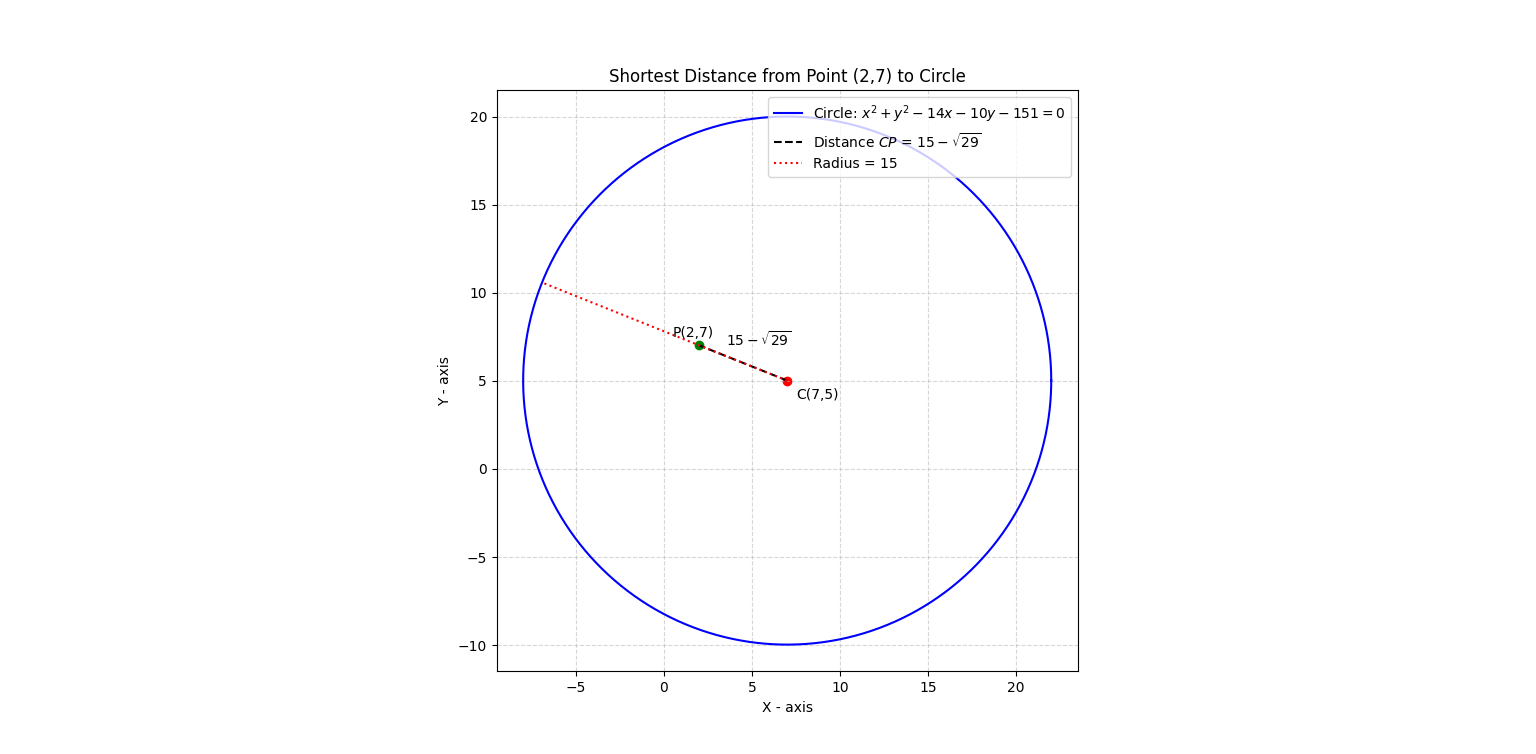
\includegraphics[width=\columnwidth]{../figs/figure_py.png}
        \caption{Shortest Distance from Point (2,7) to Circle}
        \label{fig:fig}
    \end{figure}
\end{frame}
\end{document}
